\documentclass[journal]{IEEEtran}
% *** CITATION PACKAGES ***
\usepackage{cite}

% *** GRAPHICS RELATED PACKAGES ***
%
\usepackage[pdftex]{graphicx}

% *** MATH PACKAGES ***
\usepackage{amsmath}
\interdisplaylinepenalty=2500
\usepackage{cases}

% *** SPECIALIZED LIST PACKAGES ***
% to write algorithms in the corpus of the report
\usepackage{algorithmic}

% *** PDF, URL AND HYPERLINK PACKAGES ***
\usepackage{url}

% correct bad hyndenation here
\hyphenation{op-tical net-works semi-conduc-tor}

% *** TABLES ***
\usepackage[para]{threeparttable}
\usepackage{lipsum} % filler text
\usepackage{float}
\usepackage{tabularx}
\usepackage{makecell}
\usepackage{multirow}

% to use \degree
\usepackage{gensymb}

% to use \nth 
\usepackage[super]{nth}



\begin{document}
%\lipsum[1] % filler text

\title{Dual-Objective Scheduling of Rescue Vehicles to\\
Distinguish Forest Fires via Differential Evolution\\
and Particle Swarm Optimization\\
Combined Algorithm}

\author{Guidolin Davide,
        Guglielmi Matteo\\Department of Information Engineering and Computer Science\\University of Trento, Italy\\
\texttt{davide.guidolin@studenti.unitn.it}, \texttt{matteo.guglielmi@studenti.unitn.it}}%

% The paper headers
\markboth{University of Trento, Bio-Inspired AI, September~6}%
{Shell \MakeLowercase{\textit{et al.}}: Implementation of the paper "Dual-Objective Scheduling of Rescue Vehicles to 
Distinguish Forest Fires via Differential Evolution
and Particle Swarm Optimization
Combined Algorithm"}
% make the title area
\maketitle

% As a general rule, do not put math, special symbols or citations
% in the abstract or keywords.
\begin{abstract}
With the increasing issue of global warming, the problem of forest fires during the summer season is becoming more severe every year.
For this reason we decided to focus our attention on a project that could possibly deal with this problem. Our attention landed on the paper 
\textit{"Dual-Objective Scheduling of Rescue Vehicles to Distinguish Forest Fires via Differential Evolution and Particle Swarm Optimization Combined Algorithm"}
written by \textit{Guangdong Tian, Yaping Ren, and MengChu Zhou, Fellow, IEEE}. 
In this paper the authors presented a method to optimize the deployment of vehicles used to distinguish a set of fire points with the objectives of minimize the disinguishing time and the number of motorcade used. \\
Interestingly, to test this approach, it has been applied to a real-world scenario in Mt. Daxing’anling, China.\\
\end{abstract}

% Note that keywords are not normally used for peerreview papers.
\begin{IEEEkeywords}
    PSO, DE, NSGA-II, Pareto Solutions, Genetic Operators, MHDP
\end{IEEEkeywords}

\IEEEpeerreviewmaketitle

\section{Introduction}
The problem of forest fires is becoming a big issue all around the world. With the continuous rise in temperature and with the less frequent rains in summer, the number of forest fires is increasing every year. However, the number of rescue vehicles is limited and, in case of multiple fire points, deciding how many vehicles to use for each fire point is a difficult task that has to be solved very quickly. In particular, different fire points may have different weather characteristics, like the temperature and the wind speed, and different terrain characteristics, like the slope and the type of terrain, and these parameters have to be taken into account during the decision of the number of vehicles for each fire point. Finally, the distance of the fire point to the fire department and the time that each vehicle takes to extinguish a fire are very important parameters.\\
In the paper \textit{Dual-Objective Scheduling of Rescue Vehicles to Distinguish Forest Fires via Differential Evolution and Particle Swarm Optimization Combined Algorithm}\cite{fire_distinguish}, by Tian, G., Ren, Y. \& Zhou, M., the authors present a  Multi-objective Hybrid Differential-evolution and Particle-swarm-optimization (MHDP) algorithm to minimize the time spent to extinguish a fire while minimizing the total number of vehicles used.

%spiegazione fitness functions
\section{Problem Statement}
\subsection{Problem Statement}
In this work, an implementation of an emergency scheduling algorithm to solve a scheduling problem in organizing the deployment of fire engines is proposed. \\
In particular, the considered scenario focuses on forest fires whose location points may be dislocated in several areas/points even far away from each other.
As it is possible to imagine, under emergency conditions the time factor is a key aspect to consider. Indeed, when dealing with major disasters, time is an indispensable and primary factor for each decision-maker to contain risks and damages.\\

In the context of this work, the rescue time is considered to be given by the sum of the arrival time of a motorcade to a specific fire point and the extinguishing time needed to put out the flames. Since the first is related just to a matter of distance and velocity, it is reasonable to consider arrival time as a constant if pace and distance are known.
On the other hand, the extinguishing time is highly related to several fire factors such as type of fuel, wind force, terrain slope, so it requires to be carefully modelled. \\

Fire modelling is not the only concern we have in formulating this scheduling problem since it would result unrealistic to assume infinite amount of resources. Indeed, a multi-objective optimization problem has been devised in order to take into account also the number of resources (fire engines) available in the fire station.
In light of this, as a result we get an optimal emergency policy such that a certain number of fire engines are dispatched to different fire points to minimize the firefighting time and, at the same time, it tries to minimize the number of vehicle deployed and their usage. 

\subsection{Fire Spread Model}
In the purposes of this work, a fire spread model associated with natural phenomena, i.e. wind force, initial spread speed, fuel types, temperature and terrain slope is used.\\
Mathematically, it is defined as follows :
\begin{equation}
    v_S = v_0k_sk_{\varphi} k_w = v_0 k_s k_{\varphi} e^{0.1783v_w}
    \label{eq:spread_speed}
\end{equation}
where :
\begin{itemize}
    \item $v_S$ : fire spread speed
    \item $v_0$ : initial fire spread speed
    \item $k_s$ : fuel correction factor
    \item $k_w$ : wind correction factor 
    \item $k_{\varphi}$ : terrain slope correction factor 
\end{itemize}
Furthermore : 
\begin{equation}
    v_0 = aT + bw + c
    \label{eq:intial_speed}
\end{equation}
where :
\begin{itemize}
    \item T : fire point internal temperature
    \item w : wind force
    \item a, b, c : these are terrain related factors and depends on the actual fire point location
\end{itemize}
The reference values for $k_s, k_w, k_{\varphi}$ can be found respectively, in Tables \ref{tab:ks}, \ref{tab:vw}, \ref{tab:kphi}.

\subsection{Mathematical model}
Considering what has been said before, the dual-objective emergency scheduling optimization model with multi-resource constraints is formulated as follows :
\begin{equation}
    \label{eqn:f1}
    \text{Min   } f_1 = \sum_{i=1}^N t_{E_i}
\end{equation}
\begin{equation}
    \label{eqn:f2}
    \text{Min   } f_2= \sum_{j=1}^N \sum_{m=1}^M z_{0j}^m
\end{equation}
\text{s.t.}

\begin{numcases}{}
     & $K \leq \sum_{j=1}^N \sum_{m=1}^M z_{0j}^m \leq M$ \label{eqn:constraints_a}\\
     & $L_i \leq \sum_{m=1}^M z_{0i}^m \leq U_i, i=1, \dots, N$ \label{eqn:constraints_b}\\
     & $z_{0i}^m \in \{0,1\}, m=1,\dots,M , i=1,\dots, N$ \label{eqn:constraints_c}
\end{numcases}

where:
\begin{itemize}
    \item K : Lower bound of the total number of vehicles required for forest fire emergency scheduling
    \item M : Upper bound of the total number of fire engines in the fire emergency scheduling center
    \item $z_{0i}^m$ : Binary variable ($1$ if the $m-th$ fire engine is sent from point $0$ to $i$; $0$ otherwise)
    \item $L_i$ : Lower bound of the number of fire engines to the $i-th$ fire point, $i = 1,2,\dots,N$
    \item $U_i$ : Upper bound of the number of fire engines to the $i-th$ fire point, $i = 1,2,\dots,N$
\end{itemize}
% just so separate text
\mbox{}\\

\subsubsection{Objective $f_1$}
The objective $f_1$ in (\ref{eqn:f1}) aims to minimize the extinguishing time of fires which is given by the following expression :
\begin{equation}
    \label{eqn:tei}
    t_{E_i} = \dfrac{v_{S_i}\cdot t_{A_i}}{\biggr(\sum_{m=1}^M z_{0i}^m \cdot v_m - 2v_{S_i} \biggl)}
\end{equation}
where:
\begin{itemize}
    \item $t_{A_i}$ is the arrival time of vehicles to the $i$th fire point and it is defined as:
        \begin{equation}
        t_{A_i}=\dfrac{d_{0i}}{v_{0i}}, i=1,2, \dots, N
    \end{equation}
        where $d_{0i}$ and $v_{0i}$ are the distance between point $0$ and point $i$ and the average speed of the motorcade from point $0$ to $i$, respectively.
\end{itemize}

Thus, composing (\ref{eqn:f1}) and (\ref{eqn:tei}) we have:
\begin{equation}
    f_1 = \sum_{i=1}^N \dfrac{v_{S_i}\cdot t_{A_i}}{\biggr(\sum_{m=1}^M z_{0i}^m \cdot v_m - 2v_{S_i} \biggl)}
\end{equation}

\subsubsection{Objective $f_2$}
Objective $f_2$ in (\ref{eqn:f2}) aims to minimize the number of deployed vehicles.\\
The (\ref{eqn:constraints_a}) constraint ensures that the number of motorcades sent to a specific fire point is at most $M$ and, at the same time, ensures that some fire engines are sent to each fire point such that fires are extinguished (at least $K$).\\
The second constraint (\ref{eqn:constraints_b}) limits the number of vehicles sent to the $i$-th fire point and, finally, the last constraint defines that the $z$ variables can only assume binary values.\\
It is worth to mention that the \textbf{two objective are in conflict with each other}, that's because conceptually, the first objective would require a higher number of motorcades in order to faster extinguishing the fire but this is in contrast with what we are trying to do with $f_2$.\\
Based on this, the formulated model turns out to be highly non-linear since :
\begin{itemize}
    \item[a.] Equation \ref{eqn:f1} is a non-linear function and (\ref{eqn:f2}) indicates an integer programming problem
    \item[b.] fire points are multiple so as this number increases, the emergency scheduling becomes more complex.
\end{itemize}

\section{MHDP Algorithm}
Spiegazione algoritmo MHDP
\section{Implementation of MHDP}
The code for the implementation has been written in Python.
Concerning the implementation of the MHDP algorithm, we followed the pseudocodes present in the paper for : the generation of the initial population, the crossover operator
and the adjustment of infeasible solutions.
The mutation operation was easy to implement, we only needed to select two different random individuals from the pool of possible solutions and apply (\ref{eqn:pso}).
Regarding the evaluation procedure, we had to implement also the 
\textit{fast non-dominated sort} algorithm to find the Pareto fronts.

\section{Results and analysis}
The algorithm has been tested upon the same data used by the researchers in \cite{fire_distinguish}. More precisely, the used data correspond to the fire occurred in Huzhong, region located in
Mt. Daxing’anling, at $10:40$ local time on June 29, 2010. The flames hit a total of 7 fire points in that specific area. \\
For the purposes of this work, the researchers reported all the necessary parameters to calculate the objective functions. The only element that's missing is the upper bound to the number
of vehicles for each fire point ($U_i$). Since in the paper it was presented as a given parameters, we used a representative number $10$ for all the points.\\
In table \ref{tab:our_solutions} we reported the results obtained after running the algorithm 4 consecutive times. The lowest calculated time to extinguish all
the fires is $6.17$ hours, using all the vehicles, while the lowest number of vehicles used is $29$, that is the lower bound given by the authors. In the latter case, the extinguish
time is $40.04$ hours. In figure \ref{fig:pareto_results} these solutions are plot on a 2D graph with $f_1$ on the $x$ axis and $f_2$ on the $y$ axis. 
We can see that most of the solutions are concentrated between 5 and 20 hours for $f_1$ and these solutions cover almost all the values in $f_2$, so the results are satisfying. 
Our results are very similar to the ones found by the authors, however the pareto front in their experiment (Fig. \ref{fig:authors_results}) is very well distributed and 
all the runs produce very similar solutions, but we don't know if they used the same seed for the random number generator.
\begin{table}
    \centering
    \caption{PRODUCED PARETO SOLUTIONS}
    \renewcommand{\arraystretch}{1.5}
    \begin{tabular}{ |c c c c c|  }
        \hline
        Runs & Solution Number & Scheduling schemes & $f_1$ (h) & $f_2$\\
        \hline
        \multirow{9}{*}{1} & 1 & $\{5, 4, 3, 8, 7, 6, 4\}$ & 8.25  & 37 \\
                           & 2 & $\{7, 3, 4, 8, 8, 6, 4\}$ & 6.17  & 40 \\
                           & 3 & $\{5, 3, 3, 7, 6, 5, 6\}$ & 11.83 & 35 \\
                           & 4 & $\{5, 3, 3, 7, 7, 6, 3\}$ & 12.76 & 34 \\
                           & 5 & $\{5, 2, 3, 8, 6, 4, 3\}$ & 33.38 & 31 \\
                           & 6 & $\{5, 3, 3, 7, 8, 6, 4\}$ & 9.06  & 36 \\
                           & 7 & $\{7, 3, 3, 8, 7, 6, 4\}$ & 7.31  & 38 \\
                           & 8 & $\{5, 2, 3, 6, 7, 5, 4\}$ & 19.33 & 32 \\
                           & 9 & $\{6, 2, 3, 7, 7, 5, 3\}$ & 15.87 & 33 \\
        \hline
        \multirow{12}{*}{2} & 1  & $\{6, 4, 3, 8, 7, 6, 4\}$ & 7.28  & 38 \\
                           & 2  & $\{6, 3, 3, 8, 8, 6, 5\}$ & 6.71  & 39 \\
                           & 3  & $\{6, 3, 3, 9, 7, 7, 5\}$ & 6.46  & 40 \\
                           & 4  & $\{5, 2, 3, 6, 6, 4, 3\}$ & 40.04 & 29 \\
                           & 5  & $\{5, 2, 3, 7, 6, 5, 3\}$ & 18.68 & 31 \\
                           & 6  & $\{5, 3, 4, 7, 6, 6, 4\}$ & 10.76 & 35 \\
                           & 7  & $\{5, 2, 3, 7, 6, 5, 4\}$ & 15.48 & 32 \\
                           & 8  & $\{5, 3, 3, 7, 8, 6, 5\}$ & 8.67  & 37 \\
                           & 9  & $\{5, 2, 3, 6, 6, 5, 3\}$ & 24.36 & 30 \\
                           & 10 & $\{5, 2, 3, 7, 7, 5, 5\}$ & 13.26 & 34 \\
                           & 11 & $\{5, 2, 3, 7, 7, 5, 4\}$ & 13.65 & 33 \\
                           & 12 & $\{5, 3, 3, 7, 7, 5, 6\}$ & 10.00 & 36 \\
        \hline
        \multirow{10}{*}{3} & 1  & $\{6, 4, 3, 8, 7, 6, 5\}$ & 6.89  & 39 \\
                           & 2  & $\{5, 3, 3, 7, 7, 5, 3\}$ & 13.74 & 33 \\
                           & 3  & $\{5, 2, 3, 6, 6, 5, 3\}$ & 24.36 & 30 \\
                           & 4  & $\{5, 3, 4, 7, 7, 6, 4\}$ & 8.93 & 36 \\
                           & 5  & $\{5, 2, 3, 8, 7, 5, 4\}$ & 12.66 & 34 \\
                           & 6  & $\{5, 3, 3, 9, 7, 7, 4\}$ & 7.82 & 38 \\
                           & 7  & $\{5, 2, 4, 6, 6, 5, 3\}$ & 23.73 & 31 \\
                           & 8  & $\{5, 2, 3, 8, 8, 5, 4\}$ & 12.16 & 35 \\
                           & 9  & $\{6, 3, 5, 8, 7, 6, 5\}$ & 6.38 & 40 \\
                           & 10 & $\{5, 4, 4, 7, 7, 6, 4\}$ & 8.60 & 37 \\
        \hline
        \multirow{10}{*}{4} & 1  & $\{5, 2, 3, 7, 6, 5, 3\}$ & 18.68  & 31 \\
                           & 2  & $\{5, 3, 3, 7, 6, 6, 3\}$ & 14.60 & 33 \\
                           & 3  & $\{5, 3, 3, 8, 7, 5, 4\}$ & 9.56 & 35 \\
                           & 4  & $\{6, 3, 4, 8, 8, 5, 4\}$ & 7.45 & 38 \\
                           & 5  & $\{5, 4, 3, 7, 7, 7, 4\}$ & 8.88 & 37 \\
                           & 6  & $\{6, 3, 3, 7, 8, 5, 4\}$ & 9.06 & 36 \\
                           & 7  & $\{6, 4, 3, 7, 8, 6, 5\}$ & 7.37 & 39 \\
                           & 8  & $\{6, 3, 3, 9, 8, 6, 5\}$ & 6.31 & 40 \\
                           & 9  & $\{5, 2, 3, 7, 7, 5, 5\}$ & 13.26 & 34 \\
                           & 10 & $\{5, 2, 3, 7, 6, 5, 4\}$ & 15.48 & 32 \\
        \hline
    \end{tabular}
    
    \label{tab:our_solutions}
\end{table}

\begin{figure}
    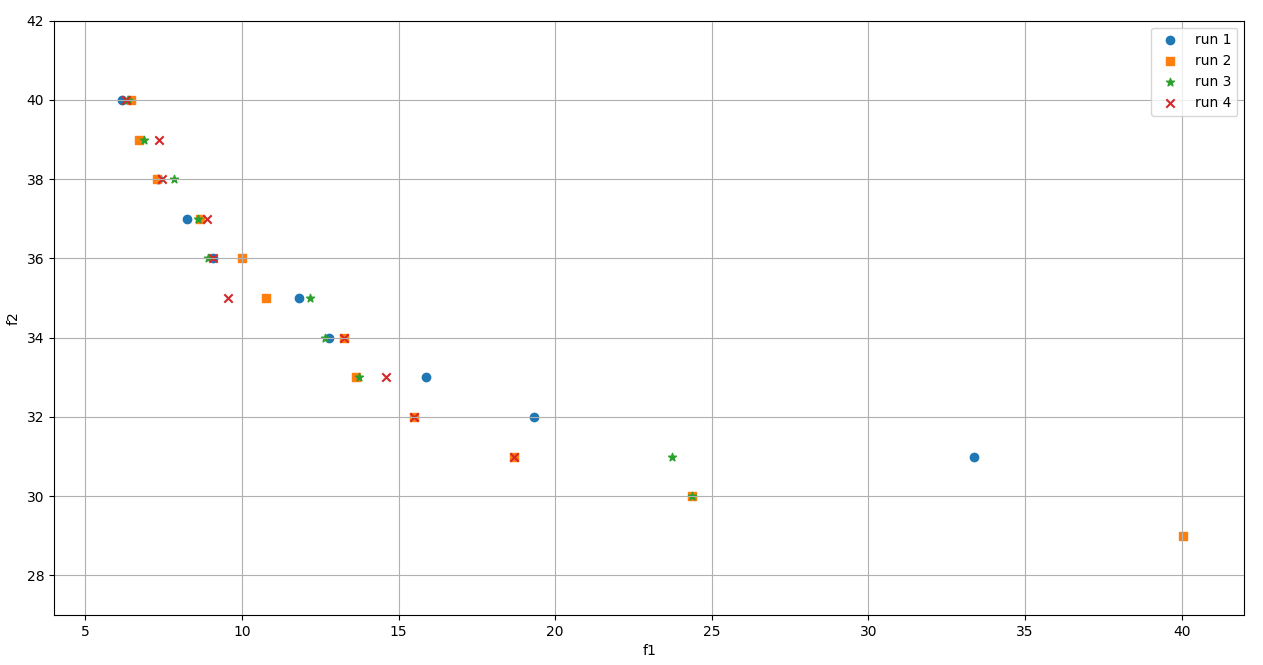
\includegraphics[width=\linewidth]{Images/our_results_4_runs.png}
    \caption{Our Pareto solutions}
    \label{fig:pareto_results}
\end{figure}

\begin{figure}
    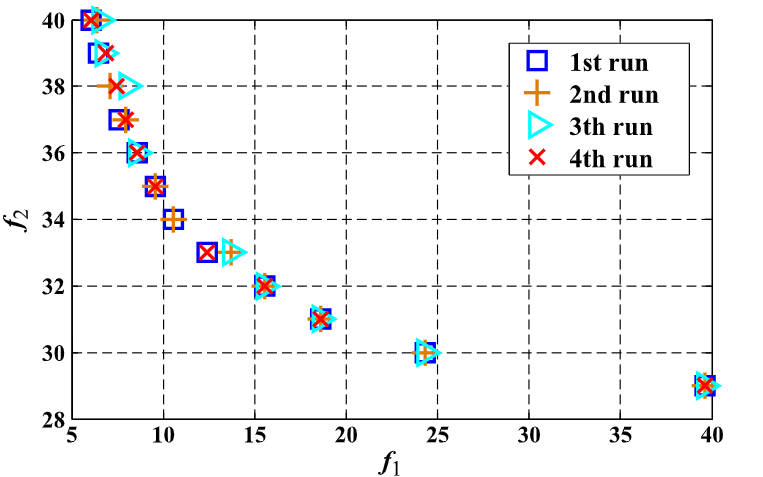
\includegraphics[width=\linewidth]{Images/authors_results.png}
    \caption{Authors' Pareto solutions}
    \label{fig:authors_results}
\end{figure}

\section{Conclusion}
Conclusioni
\section{contributions}
Davide and Matteo worked together to implement the algorithm.
Usually, for each section of the paper\cite{fire_distinguish}, we decided by chat or by a video call,
what function to implement. Then, depending on the available time, each of us
worked on the code when the other member couldn't. In this way we were able 
to review what the other did and correct possible errors or bugs.\\
Following the above procedure, Davide implemented most part of the crossover, mutation and fast non-dominated sort algorithms,
while Matteo implemented most part of the population generation, fitness computation and evaluation algorithms.
\section{Appendix}
%\begin{center}
%    \begin{threeparttable}
%        \caption{The Skewing Angles ($\beta$) for $\fam0 Mu(H)+X_2$ and
%        $\fam0 Mu(H)+HX$~\tnote{a}}
%        \begin{tabular}{rlcc}
%            \hline
%            &   & $\fam0 H(Mu)+F_2$ & $\fam0 H(Mu)+Cl_2$ \\
%            \hline
%            &$\beta$(H)  & $80.9^\circ\tnote{b}$ & $83.2^\circ$ \\
%            &$\beta$(Mu) & $86.7^\circ$ & $87.7^\circ$ \\
%            \hline
%        \end{tabular}
%        \begin{tablenotes}
%            \item[a] for the abstraction reaction, $\fam0 Mu+HX \rightarrow MuH+X$.
%            \item[b] 1 degree${} = \pi/180$ radians.
%        \end{tablenotes}
%    \end{threeparttable}

%\end{center}


\begin{center}
    \begin{threeparttable}
    \caption{$k_S$ values of different fuel types}
        \begin{tabular}{cccc}
            \hline
            \thead{Forest\\ types} & \thead{Meadow (I)} & \thead{Secondary \\forest (II)} & \thead{Coniferous \\forest (III)}\\
            \hline
            $k_s$ & $1.0$ & $0.7$ & $0.4$\\
            \hline
        \end{tabular}
        \label{tab:ks}
    \end{threeparttable}

\end{center}



\begin{center}
    \begin{threeparttable}
        \caption{$v_w$ ($k_w = e^{0.1783v_w}$) value of different wind force}
        \begin{tabular}{cc}
            \hline
            \thead{Wind force\\ level} & $v_w(m/s)$\\
            \hline
            1 & 2 \\
            2 & 3.6\\
            3 & 5.4\\
            4 & 7.4\\
            5 & 9.8\\
            6 & 12.3\\
            7 & 14.9\\
            8 & 17.7\\
            9 & 20.8\\
            10 & 24.2\\
            11 & 27.8\\
            12 & 29.8\\
            \hline
        \end{tabular}
        \label{tab:vw}
    \end{threeparttable}

\end{center}


\begin{center}
    \begin{threeparttable}
        \caption{$k_{\varphi}$ value of different terrain slopes}
        \begin{tabular}{cc}
            \hline
            Slope range & $k_{\varphi}$\\
            \hline
            $-42\degree \sim -38\degree$ & $0.007$\\
            $-37\degree \sim -33\degree$ & $0.13$\\
            $-32\degree \sim -28\degree$ & $0.21$\\
            $-27\degree \sim -23\degree$ & $0.32$\\
            $-22\degree \sim -18\degree$ & $0.46$\\
            $-17\degree \sim -13\degree$ & $0.63$\\
            $-12\degree \sim -8\degree$ & $0.83$\\
            $-7\degree \sim -3\degree$ & $0.90$\\
            $-2\degree \sim 2\degree$ & $1.00$\\
            $3\degree \sim 7\degree$ & $1.20$\\
            $8\degree \sim 12\degree$ & $1.60$\\
            $13\degree \sim 17\degree$ & $2.10$\\
            $18\degree \sim 22\degree$ & $2.90$\\
            $23\degree \sim 27\degree$ & $4.10$\\
            $28\degree \sim 32\degree$ & $6.20$\\
            $33\degree \sim 37\degree$ & $10.10$\\
            $38\degree \sim 42\degree$ & $17.50$\\
            \hline
        \end{tabular}
        \label{tab:kphi}
    \end{threeparttable}

\end{center}


\begin{table}
    \centering
    \caption{PRODUCED PARETO SOLUTIONS}
    \renewcommand{\arraystretch}{1.5}
    \begin{tabular}{ |c c c c c|  }
        \hline
        Runs & Solution Number & Scheduling schemes & $f_1$ (h) & $f_2$\\
        \hline
        \multirow{9}{*}{1} & 1 & $\{5, 4, 3, 8, 7, 6, 4\}$ & 8.25  & 37 \\
                           & 2 & $\{7, 3, 4, 8, 8, 6, 4\}$ & 6.17  & 40 \\
                           & 3 & $\{5, 3, 3, 7, 6, 5, 6\}$ & 11.83 & 35 \\
                           & 4 & $\{5, 3, 3, 7, 7, 6, 3\}$ & 12.76 & 34 \\
                           & 5 & $\{5, 2, 3, 8, 6, 4, 3\}$ & 33.38 & 31 \\
                           & 6 & $\{5, 3, 3, 7, 8, 6, 4\}$ & 9.06  & 36 \\
                           & 7 & $\{7, 3, 3, 8, 7, 6, 4\}$ & 7.31  & 38 \\
                           & 8 & $\{5, 2, 3, 6, 7, 5, 4\}$ & 19.33 & 32 \\
                           & 9 & $\{6, 2, 3, 7, 7, 5, 3\}$ & 15.87 & 33 \\
        \hline
        \multirow{12}{*}{2} & 1  & $\{6, 4, 3, 8, 7, 6, 4\}$ & 7.28  & 38 \\
                           & 2  & $\{6, 3, 3, 8, 8, 6, 5\}$ & 6.71  & 39 \\
                           & 3  & $\{6, 3, 3, 9, 7, 7, 5\}$ & 6.46  & 40 \\
                           & 4  & $\{5, 2, 3, 6, 6, 4, 3\}$ & 40.04 & 29 \\
                           & 5  & $\{5, 2, 3, 7, 6, 5, 3\}$ & 18.68 & 31 \\
                           & 6  & $\{5, 3, 4, 7, 6, 6, 4\}$ & 10.76 & 35 \\
                           & 7  & $\{5, 2, 3, 7, 6, 5, 4\}$ & 15.48 & 32 \\
                           & 8  & $\{5, 3, 3, 7, 8, 6, 5\}$ & 8.67  & 37 \\
                           & 9  & $\{5, 2, 3, 6, 6, 5, 3\}$ & 24.36 & 30 \\
                           & 10 & $\{5, 2, 3, 7, 7, 5, 5\}$ & 13.26 & 34 \\
                           & 11 & $\{5, 2, 3, 7, 7, 5, 4\}$ & 13.65 & 33 \\
                           & 12 & $\{5, 3, 3, 7, 7, 5, 6\}$ & 10.00 & 36 \\
        \hline
        \multirow{10}{*}{3} & 1  & $\{6, 4, 3, 8, 7, 6, 5\}$ & 6.89  & 39 \\
                           & 2  & $\{5, 3, 3, 7, 7, 5, 3\}$ & 13.74 & 33 \\
                           & 3  & $\{5, 2, 3, 6, 6, 5, 3\}$ & 24.36 & 30 \\
                           & 4  & $\{5, 3, 4, 7, 7, 6, 4\}$ & 8.93 & 36 \\
                           & 5  & $\{5, 2, 3, 8, 7, 5, 4\}$ & 12.66 & 34 \\
                           & 6  & $\{5, 3, 3, 9, 7, 7, 4\}$ & 7.82 & 38 \\
                           & 7  & $\{5, 2, 4, 6, 6, 5, 3\}$ & 23.73 & 31 \\
                           & 8  & $\{5, 2, 3, 8, 8, 5, 4\}$ & 12.16 & 35 \\
                           & 9  & $\{6, 3, 5, 8, 7, 6, 5\}$ & 6.38 & 40 \\
                           & 10 & $\{5, 4, 4, 7, 7, 6, 4\}$ & 8.60 & 37 \\
        \hline
        \multirow{10}{*}{4} & 1  & $\{5, 2, 3, 7, 6, 5, 3\}$ & 18.68  & 31 \\
                           & 2  & $\{5, 3, 3, 7, 6, 6, 3\}$ & 14.60 & 33 \\
                           & 3  & $\{5, 3, 3, 8, 7, 5, 4\}$ & 9.56 & 35 \\
                           & 4  & $\{6, 3, 4, 8, 8, 5, 4\}$ & 7.45 & 38 \\
                           & 5  & $\{5, 4, 3, 7, 7, 7, 4\}$ & 8.88 & 37 \\
                           & 6  & $\{6, 3, 3, 7, 8, 5, 4\}$ & 9.06 & 36 \\
                           & 7  & $\{6, 4, 3, 7, 8, 6, 5\}$ & 7.37 & 39 \\
                           & 8  & $\{6, 3, 3, 9, 8, 6, 5\}$ & 6.31 & 40 \\
                           & 9  & $\{5, 2, 3, 7, 7, 5, 5\}$ & 13.26 & 34 \\
                           & 10 & $\{5, 2, 3, 7, 6, 5, 4\}$ & 15.48 & 32 \\
        \hline
    \end{tabular}
    
    \label{tab:our_solutions}
\end{table}

\newpage
\begin{thebibliography}{1}

\bibitem{IEEEhowto:kopka}
H.~Kopka and P.~W. Daly, \emph{A Guide to \LaTeX}, 3rd~ed.\hskip 1em plus
  0.5em minus 0.4em\relax Harlow, England: Addison-Wesley, 1999.

\end{thebibliography}


\end{document}


